% !TEX root = ../thesis.tex

\chapter{Erstellung eines featurebasierten Datensets}

\paragraph{Ausblick:}
Dieses Kapitel widmet sich der schrittweisen Erläuterung des Prozesses zur Erstellung des featurebasierten Datensets, welches zur Anlernung der Machine-Learning-Klassifikatoren dient. Dazu wird zunächst die Datenauswahl näher beleuchtet. Darauf folgt eine Darlegung der Konstruktion des Datensets sowie der Auswahl und Berechnung der Metriken, welche als Attribute (Features) im Rahmen der Anlernung der Klassifikatoren dienen.
\\
\hrule

\section{Datenauswahl}

Wie im vorangegangenen Kapitel bereits erwähnt wurde, bildet das Datenset die Grundlage für die Anlernung der Machine-Learning-Klassifikatoren und wird eigens für diese Arbeit auf Basis von Commits von 13 featurebasierten Software-Projekten erstellt. Die Auswahl der Software-Projekte erfolge anhand von vorheriger Verwendung in wissenschaftlicher Literatur \cite{Hunsen2015,Liebig2010,Queiroz2016}. Die für diese Arbeit verwendeten Software-Projekte sind samt ihres Einsatzzweckes und ihrer Datenquellen in Tabelle XX aufgeführt.

\begin{table}
\centering
\caption{Übersicht der verwendeten Software-Projekten\protect\footnotemark{}}
\label{tab:tools}
\resizebox{\linewidth}{!}{%
\begin{tabular}{|l|c|c|l|c|c|} 
\cline{2-3}\cline{5-6}
\multicolumn{1}{l|}{} & \textbf{Zweck}       & \textbf{Datenquelle}  &                      & \textbf{Zweck}       & \textbf{Datenquelle}     \\ 
\hline
\textbf{Blender}      & 3D-Modellierungstool & GitHub-Mirror         & \textbf{libxml2}     & XML-Parser           & GitLab-Repository        \\ 
\hline
\textbf{Busybox}      & UNIX-Toolkit         & Git-Repository        & \textbf{lighttpd}    & Webserver            & Git-Repository           \\ 
\hline
\textbf{Emacs}        & Texteditor           & GitHub-Mirror         & \textbf{MPSolve}     & Polynomlöser         & GitHub-Repository        \\ 
\hline
\textbf{GIMP}         & Bildbearbeitung      & GitLab-Repository     & \textbf{Parrot}      & virtuelle Maschine   & GitHub-Repository        \\ 
\hline
\textbf{Gnumeric}     & Tabellenkalkulation  & GitLab-Repository     & \textbf{Vim}         & Texteditor           & GitHub-Repository        \\ 
\hline
\textbf{gnuplot}      & Plotting-Tool        & GitHub-Mirror         & \textbf{xfig}        & Grafikeditor         & Sourceforge-Repository~  \\ 
\hline
\textbf{Irssi}        & IRC-Client           & GitHub-Repository     & \multicolumn{1}{l}{} & \multicolumn{1}{l}{} & \multicolumn{1}{l}{}     \\
\cline{1-3}
\end{tabular}
}
\end{table}
\footnotetext{Links zu den Websites der Softwareprojekte und deren Repositories können im \hyperref[appendix1]{Anhang} eingesehen werden.}

Zum Erhalt der Commit-Daten der Software-Projekte wurde die Python-Library PyDriller\footnote{\href{https://github.com/ishepard/pydriller}{https://github.com/ishepard/pydriller}} verwendet \cite{Spadini2018}. Diese ermöglicht eine einfache Datenextraktion von Git-Repositories zum Erhalt von Commits, Commit-Nachrichten, Entwicklern, Diffs und mehr. Ein beispielhafter Sourcecode-Ausschnitt zur Konsolenausgabe von Metadaten eines Commits (Autor, Name der veränderten Dateien, Typ der Veränderung und jeweilige zyklomatische Komplexität der Dateien) ist in Listing 3.1 aufgeführt. 

\begin{lstlisting}[language=Python, caption=Beispielhafter PyDriller-Code zur Ausgabe von Metadaten von Commits, frame=single]
for commit in RepositoryMining("link_to_repo").traverse_commits(): 
	for m in commit.modifications: 
		print( 
		     "Author {}".format(commit.author.name), 
		     " modified {}".format(m.filename), 
		     " with a change type of {}".format(m.change_type.name), 
		     " and the complexity is {}".format(m.complexity) 
		)
\end{lstlisting}

Als Input der Python-Scripte zum Erhalt der Commit-Daten dienten jeweils die URLs zu den Git-Repositories der Software-Projekte. Weiterhin wurden die Daten in Commits je Release aufgeteilt. Durchgeführt wurde dies durch die Angabe von Release-Tags, basierend auf der Tag-Struktur von Git-Repositories, im PyDriller-Code. Für jede veränderte Datei innerhalb eines Commits und eines Releases wurden die folgenden Metadaten mit Hilfe von PyDriller abgerufen:

\begin{multicols}{2}
\begin{itemize}
\item Commit-Hash (eindeutiger Bezeichner des zugehörigen Commits)
\item Autor des zugehörigen Commits
\item zugehörige Commit-Nachricht
\item Name der veränderten Datei
\item Lines-of-Code der veränderten Datei
\item zyklomatische Komplexität der veränderten Datei
\item Anzahl der hinzugefügten Zeilen zur Datei
\item Anzahl der entfernten Zeilen von der Datei
\item Art der Änderung (ADD, REM, MOD)\footnote{Diese Information fand in der weiteren Erstellung des Datensets keine Verwendung.}
\item Diff der Veränderung
\end{itemize}
\end{multicols}

Die auf diese Weise erhaltenen Daten wurden nach dem Abruf in einer MySQL-Datenbank gespeichert. Für jedes Software-Projekt wurde eine eigene Tabelle erstellt, in welcher neben der oben stehenden Metadaten zudem der Name des betreffenden Software-Projekts und die den Commits zugehörigen Release-Nummern gespeichert wurden. Jede veränderte Datei eines Commits erhält eine Zeile der Datenbank-Tabellen. In Tabelle XX kann eingesehen werden wie viele Releases je Software-Projekt zum Abruf einbezogen wurden und wie viele Commits daraus resultieren.

\begin{table}
\centering
\caption{Übersicht der Anzahl der Releases und Commits je Software-Projekt}
\label{tab:tools}
\resizebox{\linewidth}{!}{%
\begin{tabular}{|l|c|c|l|c|c|} 
\cline{2-3}\cline{5-6}
\multicolumn{1}{l|}{} & \textbf{\#Releases}  & \textbf{\#Commits}  &                      & \multicolumn{1}{l|}{\textbf{\#Releases}~} & \textbf{\#Commits}~   \\ 
\hline
\textbf{Blender}      & 11                   & 19119               & \textbf{libxml2}     & 10                                        & 732                   \\ 
\hline
\textbf{Busybox}      & 14                   & 4984                & \textbf{lighttpd}    & 6                                         & 2597                  \\ 
\hline
\textbf{Emacs}        & 7                    & 12805               & \textbf{MPSolve}     & 8                                         & 668                   \\ 
\hline
\textbf{GIMP}         & 14                   & 7240                & \textbf{Parrot}      & 7                                         & 16245                 \\ 
\hline
\textbf{Gnumeric}     & 8                    & 6025                & \textbf{Vim}         & 7                                         & 9849                  \\ 
\hline
\textbf{gnuplot}      & 5                    & 6619                & \textbf{xfig}        & 7                                         & 18                    \\ 
\hline
\textbf{Irssi}        & 7                    & 253                 & \multicolumn{1}{l}{} & \multicolumn{1}{l}{}                      & \multicolumn{1}{l}{}  \\
\cline{1-3}
\end{tabular}
}
\end{table}

Diese \glqq Rohdaten\grqq{} dienen zur weiteren Verarbeitung hinsichtlich der Erstellung des Datensets und der anschließenden Berechnung der Metriken. Eine Erläuterung der weiteren Verarbeitung der Daten folgt im kommenden Abschnitt.

\begin{table}[]
\caption[Caption for LOF]{Übersicht der zur Erstellung des Datensets verwendeten Software-Projekten mit zugehörigen Werten}
\label{tab:tools}
\resizebox{\textwidth}{!}{%
\begin{tabular}{lccccccc}
                                       & \textbf{Zweck}       & \textbf{Datenquelle}   & \textbf{\#Releases} & \textbf{\#Commits} & \textbf{\#Korrektiv} & \textbf{\#Fehlereinführend} & \textbf{\#Features} \\ \hline
\multicolumn{1}{l|}{\textbf{Blender}}  & 3D-Modellierungstool & GitHub-Mirror          & 11                  & 19119              & 8258                 & 1418                        & 4637         \\
\multicolumn{1}{l|}{\textbf{Busybox}}  & UNIX-Toolkit         & Git-Repository         & 14                  & 4984               & 1408                 & 142                         & 702                 \\
\multicolumn{1}{l|}{\textbf{Emacs}}    & Texteditor           & GitHub-Mirror          & 7                   & 12805              & 6959                 & 685                         & 863                 \\
\multicolumn{1}{l|}{\textbf{GIMP}}     & Bildbearbeitung      & GitLab-Repository      & 14                  & 7240               & 1703                 & 272                         & 1620                \\
\multicolumn{1}{l|}{\textbf{Gnumeric}} & Tabellenkalkulation  & GitLab-Repository      & 8                   & 6025               & 1591                 & 136                         & 725                 \\
\multicolumn{1}{l|}{\textbf{gnuplot}}  & Plotting-Tool        & GitHub-Mirror          & 5                   & 6619               & 880                  & 1323                        & 625                 \\
\multicolumn{1}{l|}{\textbf{Irssi}}    & IRC-Client           & GitHub-Repository      & 7                   & 253                & 77                   & 1                           & 17                  \\
\multicolumn{1}{l|}{\textbf{libxml2}}  & XML-Parser           & GitLab-Repository      & 10                  & 732                & 409                  & 37                          & 225                 \\
\multicolumn{1}{l|}{\textbf{lighttpd}} & Webserver            & Git-Repository         & 6                   & 2597               & 1202                 & 555                         & 323                 \\
\multicolumn{1}{l|}{\textbf{MPSolve}}  & Polynomlöser         & GitHub-Repository      & 8                   & 668                & 158                  & 69                          & 130                 \\
\multicolumn{1}{l|}{\textbf{Parrot}}   & Virtuelle Maschine   & GitHub-Repository      & 7                   & 16245              & 3437                 & 824                         & 559                 \\
\multicolumn{1}{l|}{\textbf{Vim}}      & Texteditor           & GitHub-Repository      & 7                   & 9849               & 1033                 & 2571                        & 1227                \\
\multicolumn{1}{l|}{\textbf{xfig}}     & Grafikeditor         & Sourceforge-Repository & 7                   & 18                 & 0                    & 0                           & 205                
\end{tabular}%
}
\end{table}

\section{Konstruktion des Datensets}

Die Konstruktion des Datensets gliedert sich in mehrere Phasen der Datenverarbeitung und -optimierung. Die erste Phase besteht aus der Extraktion der involvierten Features einer veränderten Datei. Dazu wurden mithilfe eines Python-Scripts die sogenannten Präprozessor-Direktiven \texttt{\#IFDEF} und \texttt{\#IFNDEF} in den Diffs der veränderten Dateien identifiziert und anschließend die den Direktiven folgende Zeichenfolge bis zum Ende der Codezeile als Feature gespeichert. Die Identifizierung erfolgte mittels regulären Ausdrücken. Gespeichert werden die pro Datei identifizierten Features in einer zusätzlichen Spalte in den jeweiligen MySQL-Tabellen der Software-Projekte. Konnte kein Feature identifiziert werden, wird entsprechend \texttt{none} gepseichert.

Dieser Weg der Identifizierung birgt einige Hindernisse. Diese können, neben dem Normalfall, in Abbildung XX gesehen werden. In einigen C-Programmierparadigmen ist es üblich, Header-Dateien mittels Präprozessor-Direktiven in Sourcecode einzubinden, sodass sie wie Features scheinen (siehe erster unerwünschter Fall in Abbildung XX). Diese "Header-Features", wie sie im weiteren Verlauf genannt werden, sollten jedoch ignoriert werden, da sie im Sourcecode keine Variabilität erzeugen. In der Regel sind diese Header-Features identifizierbar durch ihre Namensgebung in Form eines angehängten \texttt{\_h\_} an den Featurenamen, wie beispielsweise \texttt{featurename\_h\_}. Dieser angehängte Teil erlaubt es, die Header-Features mittels regulärer Ausdrücke zu erkennen und auszufiltern. 

Ebenfalls besteht die Möglichkeit, dass "falsche" Features identifiziert werden können. Beispiele dafür können von \texttt{\#IFDEFs} stammen, welche in Kommentaren verwendet wurden (siehe zweiter unerwünschter Fall in Abbildung XX). Solche falschen Features wurden in einer manuellen Sichtung der identifizierten Features entfernt und durch \texttt{none} ersetzt.

\begin{figure}[]
    \centering
    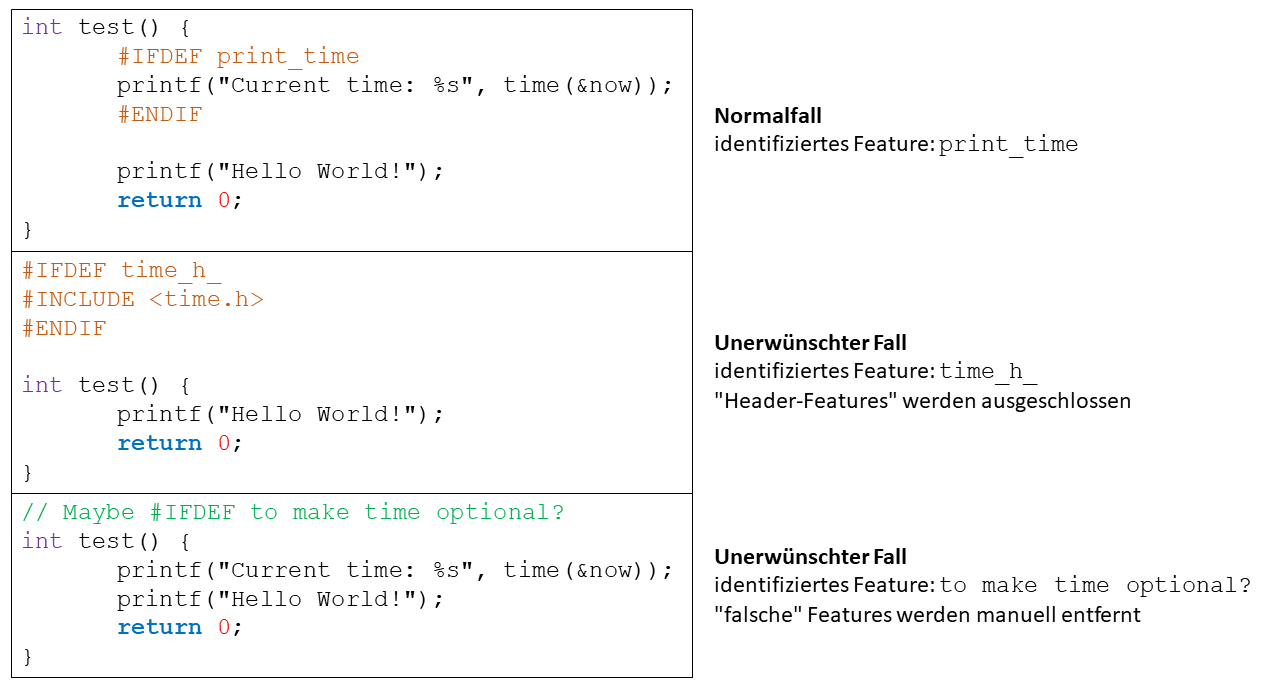
\includegraphics[width=\textwidth]{images/Features}
    \caption{Normalfall und unerwünschte Fälle bei der Identifizierung von Features\label{fig:feat}}
\end{figure}

Die nächste Phase der Verarbeitung besteht aus der Identifizierung von korrektiven Commits. Eine dafür gängige Methode, die auch in dieser Arbeit Anwendung fand, besteht aus der Analyse der Commit-Nachrichten auf das Vorhandensein von bestimmten Schlagworten (\textbf{HIER ANGABE ZU LITERATUR AUS RODRIGO}). Bei den Schlagworten handelt es sich um \glqq bug\grqq, \glqq error\grqq, \glqq fail\grqq{} und \glqq fix\grqq. 

\textbf{HIER!}

\begin{table}[]
\caption{Übersicht des Schemas der Haupttabellen des Datensets}
\label{tab:schema1}
\resizebox{\textwidth}{!}{%
\begin{tabular}{ll|ll}
\textbf{Spaltenname} & \textbf{Beschreibung}                                                                              & \textbf{Spaltenname} & \textbf{Beschreibung}                                                                           \\ \hline
name                 & Name des Softwareprojekts                                                                          & lines\_added         & \begin{tabular}[c]{@{}l@{}}Anzahl der hinzugefügten Zeilen\\ zur geänderten Datei\end{tabular}  \\
release\_number      & \begin{tabular}[c]{@{}l@{}}zugehörige Release-Version\\ basierend auf vergebenen Tags\end{tabular} & lines\_removed       & \begin{tabular}[c]{@{}l@{}}Anzahl der entfernten Zeilen\\ von der geänderten Datei\end{tabular} \\
commit\_hash         & \begin{tabular}[c]{@{}l@{}}eindeutiger Bezeichner eines \\ Commits\end{tabular}                    & change\_type         & Art der Änderung                                                                                \\
commit\_author       & Autor eines Commits                                                                                & diff                 & Diff der geänderten Datei                                                                       \\
commit\_msg          & Nachricht eines Commits                                                                            & corrective           & \begin{tabular}[c]{@{}l@{}}Indikator, ob Commit\\ fehlerbehebend war\end{tabular}               \\
filename             & Name der geänderten Datei                                                                          & bug\_introducing     & \begin{tabular}[c]{@{}l@{}}Indikator, ob Commit\\ fehlereinführend war\end{tabular}             \\
nloc                 & \begin{tabular}[c]{@{}l@{}} \glqq Lines of code\grqq{} der geänderten\\ Datei\end{tabular}                     & feature              & \begin{tabular}[c]{@{}l@{}}Namen der zugehörigen Features\\ der geänderten Datei\end{tabular}   \\
cycomplexity         & \begin{tabular}[c]{@{}l@{}}Zyklomatische Komplexität\\ der geänderten Datei\end{tabular}           &                      &                                                                                                
\end{tabular}%
}
\end{table}

\begin{table}[]
\caption{Übersicht des Schemas der SZZ-Tabellen des Datensets}
\label{tab:schema3}
\resizebox{\textwidth}{!}{%
\begin{tabular}{ll|ll}
\textbf{Spaltenname} & \textbf{Beschreibung}                                                            & \textbf{Spaltenname} & \textbf{Beschreibung}                                                                     \\ \hline
name                 & Name des Softwareprojekts                                                        & filename             & einem Commit zugehörige Dateien                                                           \\
commit\_hash         & \begin{tabular}[c]{@{}l@{}}Commit-Hashes fehlerbehebender\\ Commits\end{tabular} & bug\_introducing     & \begin{tabular}[c]{@{}l@{}}Auflistung der fehlereinführenden\\ Commit-Hashes\end{tabular} \\
filepath             & einem Commit zugehörige Dateipfade                                               &                      &                                                                                          
\end{tabular}%
}
\end{table}

\section{Metriken}

\textbf{Ergänzen!!!!}

\begin{table}[]
\caption{Übersicht des Schemas der Metrics-Tabellen des Datensets}
\label{tab:schema2}
\resizebox{\textwidth}{!}{%
\begin{tabular}{ll|ll}
\textbf{Spaltenname} & \textbf{Beschreibung}                                                                                                                                                                          & \textbf{Spaltenname} & \textbf{Beschreibung}                                                                                                                                                           \\ \hline
name                 & Name des Softwareprojekts                                                                                                                                                                      & oexp                 & \begin{tabular}[c]{@{}l@{}}"Erfahrung" des Entwicklers, der am\\ meisten zum betreffenden Feature / \\ zur betreffenden Datei in  einem Release \\ beigetragen hat\end{tabular} \\
release\_number      & \begin{tabular}[c]{@{}l@{}}zugehörige Release-Version\\ basierend auf vergebene Tags\end{tabular}                                                                                              & scat                 & \begin{tabular}[c]{@{}l@{}}Scattering Degree des betreffenden Features / \\ der betreffenden Datei\end{tabular}                                                                 \\
feature / filename   & \begin{tabular}[c]{@{}l@{}}betreffendes Feature / \\ betreffende Datei\end{tabular}                                                                                                            & tang                 & \begin{tabular}[c]{@{}l@{}}Tangling Degree des betreffenden Features / \\ der betreffenden Datei\end{tabular}                                                                   \\
comm                 & \begin{tabular}[c]{@{}l@{}}Anzahl der Commits, die in einem\\ Release dem betreffenden Feature / \\ der betroffenen Datei gewidmet sind\end{tabular}                                           & nloc                 & \begin{tabular}[c]{@{}l@{}}Durchschnittliche Lines of Code der Bearbeitungen \\ des betreffenden Features / der betreffenden Datei\\ in einem Release\end{tabular}              \\
adev                 & \begin{tabular}[c]{@{}l@{}}Anzahl der Entwickler, die das\\ betreffende Feature / die betreffende \\ Datei in einem Release bearbeitet haben\end{tabular}                                      & cyco                 & \begin{tabular}[c]{@{}l@{}}Durchschnittliche zyklomatische Komplexität der \\ Bearbeitungen  des betreffenden Features /\\ der betreffenden Datei in einem Release\end{tabular} \\
ddev                 & \begin{tabular}[c]{@{}l@{}}kummulierte Anzahl der Entwickler, \\ die das betreffende Feature / \\ die betreffende Datei in einem\\ Release bearbeitet haben\end{tabular}                       & addl                 & \begin{tabular}[c]{@{}l@{}}Durchschnittliche Anzahl der hinzugefügten Zeilen \\ des betreffenden Features / der betreffenden Datei\\ in einem Release\end{tabular}              \\
exp                  & \begin{tabular}[c]{@{}l@{}}Geometrisches Mittel der "Erfahrung"\\ aller Entwickler, die am betreffenden\\ Feature / an der betreffenden Datei\\ in einem Release gearbeitet haben\end{tabular} & reml                 & \begin{tabular}[c]{@{}l@{}}Durchschnittliche Anzahl der entfernten Zeilen \\ des betreffenden Features / der betreffenden Datei\\ in einem Release\end{tabular}                
\end{tabular}%
}
\end{table}

\cleardoublepage